\providecommand{\fn}[1]{\ensuremath{f\left(#1\right)}}
\providecommand{\e}[1]{\ensuremath{E\left(#1\right)}}
% A continuous random variable $X$ has a probability density function 
% $\fn{x} = e^{-x}$,$0<x<\infty$. Then $P(X > 1)$ is

% \section{Solution}
Given,
\begin{align} \label{14:1}
\fn{x} = e^{-x} , 0<x<\infty
\end{align}
We have to find \pr{X>1},
\begin{align}
\pr{X>1} = \int_{1}^{\infty}{\fn{x}}\,dx\label{14:2}
\end{align}
Using \eqref{14:1} in \eqref{14:2}
\begin{align}
\pr{X>1} &= \int_{1}^{\infty}{e^{-x}}\,dx\\
&= \left[-e^{-x}\right]_1^{\infty}\\
&= (-e^{-\infty}) - (-e^{-1})\\
&= e^{-1}\\
&= \frac{1}{e}\\
 \implies \pr{X>1} &= 0.368
\end{align}
Finding the probability using uniform distribution,

Let $F_X(x)$ be the cumulative distribution function of random variable X.
\begin{align}
    F_X(x)=\int_{0}^x \fn{x} dx\label{14:x}
\end{align}
$F_X(x)$ can be obtained from the uniform distribution of a random variable U on (0,1) and let U=$e^{-x}$. 
\begin{align}
    0 < U < 1
\end{align}
As for random variable X also,
\begin{align}
    0 < F_X(x) < 1
\end{align}
This similarity between U and $F_X(x)$ is used to generate the random variable X from U.
\begin{align}
    F_X(x)&=\pr{X<x}\\
    &=\pr{-\log_e U<x}\\
    &=\pr{U<e^{-x}}\\
    &=F_U(e^{-x})\label{14:y}
\end{align}
From uniform distribution,
\begin{align}
    F_U(x)= x ,0<x<1 \label{14:z}
\end{align}
\begin{figure}[htp]
    \centering
    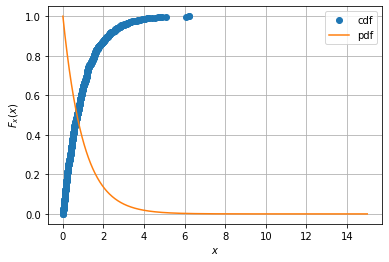
\includegraphics[width=\columnwidth]{solutions/ec/14/FIGURES/Figure.png}
    \caption{CDF  of random variable X}
\label{14:fig:CDF}
\end{figure}
In the figure \ref{14:fig:CDF},orange colour graph represents the pdf of the random variable X and blue colour graph represents the cdf of the random variable X.
Using \eqref{14:z} in \eqref{14:y},
Cumulative distribution function (CDF) of random variable X is,
\begin{align}
F_X(x) &= \pr{X<x}\\
&= 1 -e^{-x} ,0<x<\infty \label{14:g}
\end{align}
Now we have to find \pr{X>1},
\begin{align}
    \pr{X>1} &= 1-\pr{X<1}
\end{align}
Using  \eqref{14:g},
\begin{align}
    \pr{X>1} &= 1-(1 -e^{-1})\\
    \pr{X>1} &= e^{-1}\\
   \implies \pr{X>1} &= 0.368 
\end{align}

%\end{document}
